\section{Sistema}

Apresentar o texto e as imagens referente ao sistema desenvolvido explicitando as
funcionalidades desenvolvidas.

% Exemplo de inserção de figura com subfiguras
\begin{figure}[htbp]
\centering
    \begin{subfigure}[b]{7cm}
        \centering
        % Primeira subfigura
        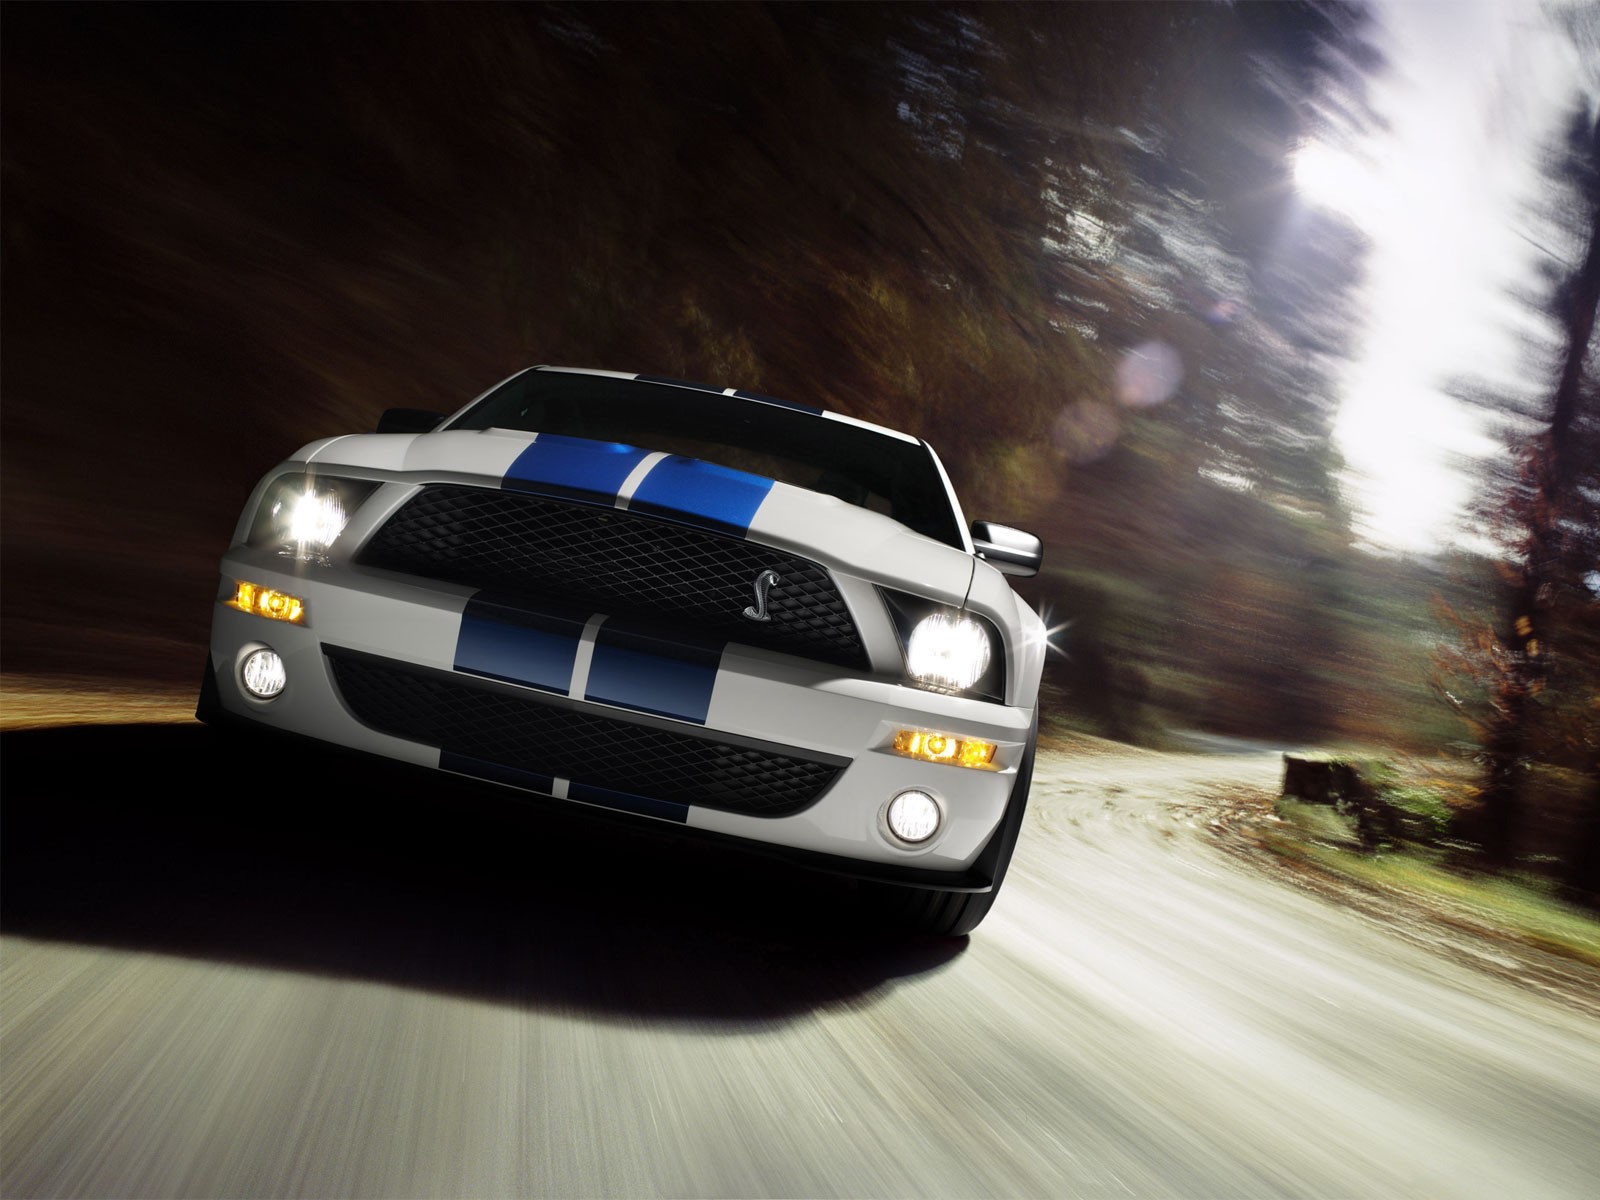
\includegraphics[width=7cm]{anexos/sub1fig2.jpg} % URI da subfigura
        \subcaption{
        % Legenda da subfigura
        Carro branco.
        }
        \label{fig2:sub1}
    \end{subfigure}
\quad
    \begin{subfigure}[b]{7cm}
        \centering
        % Segunda subfigura
        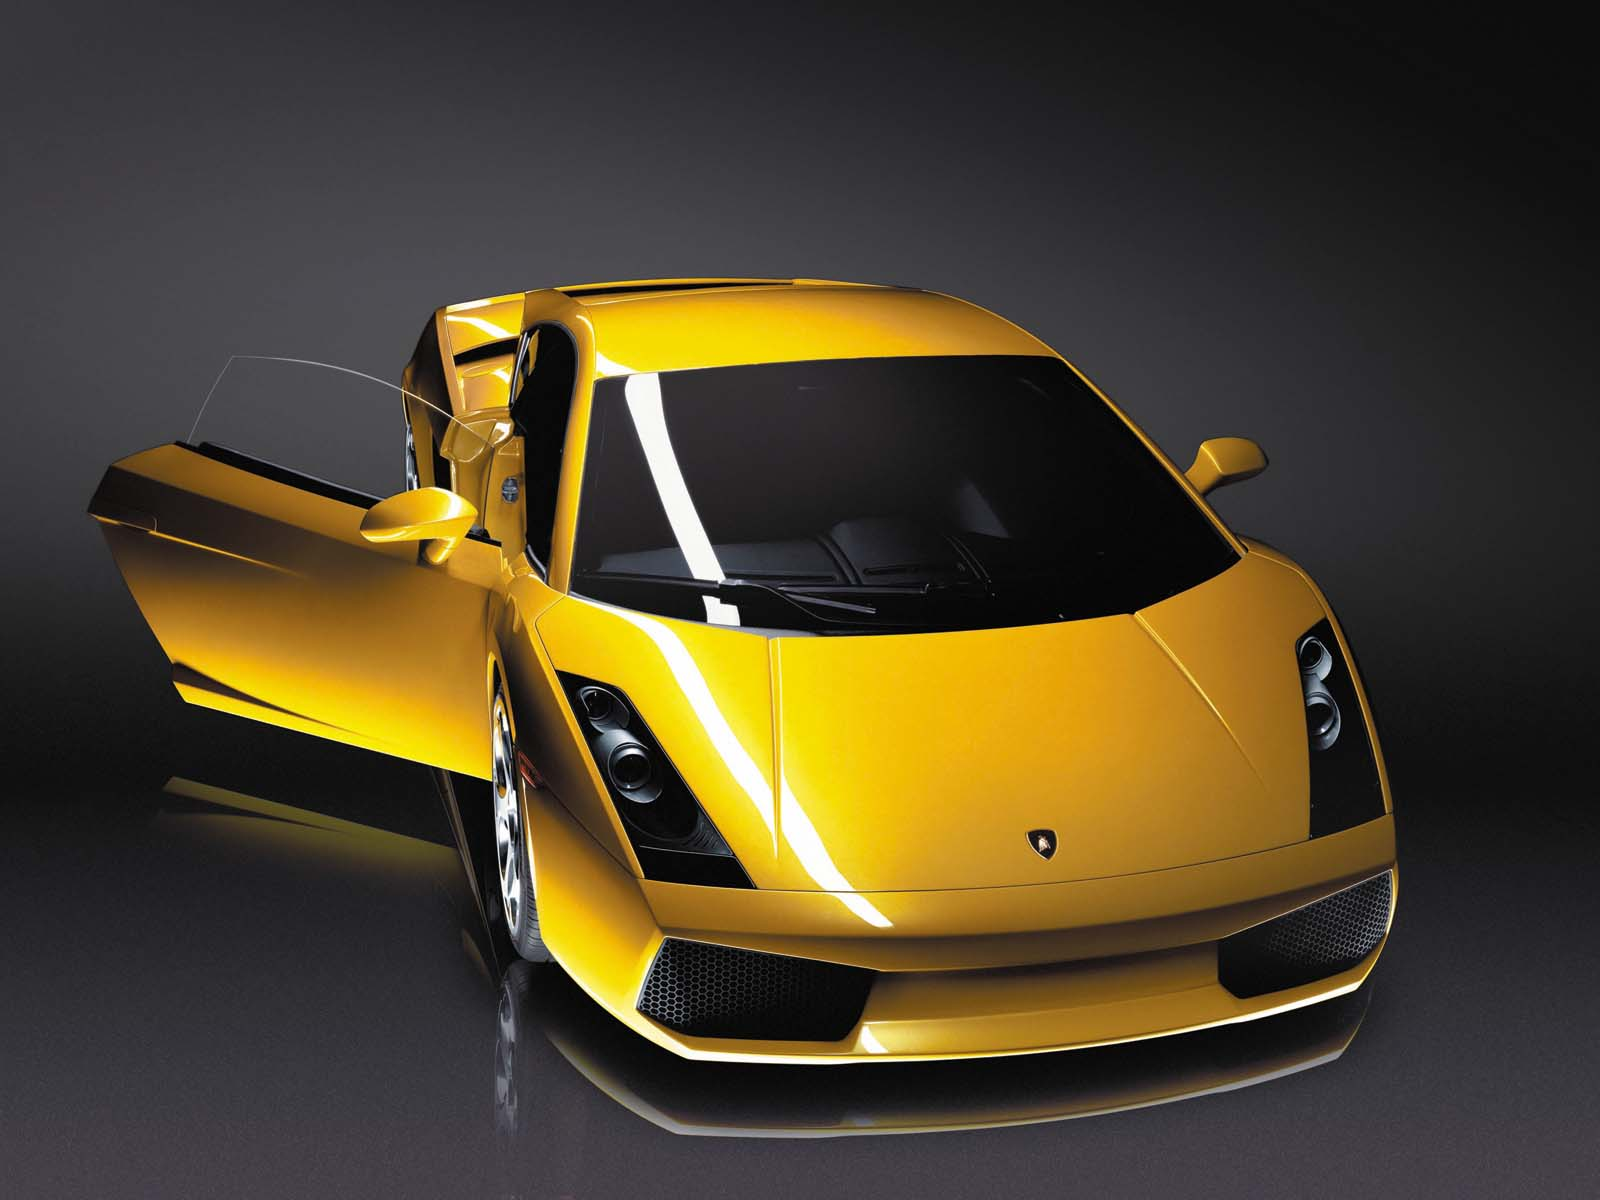
\includegraphics[width=7cm]{anexos/sub2fig2.jpg} % URI da subfigura
        \subcaption{
        % Legenda da subfigura
        Carro amarelo.
        }
        \label{fig2:sub2}
    \end{subfigure}
\caption{
Legenda da figura.
}
\label{fig:fig2} % Tag para referência
\end{figure}